\documentclass{article}

% if you need to pass options to natbib, use, e.g.:
\PassOptionsToPackage{sort}{natbib}
% before loading neurips_2019

% ready for submission
% \usepackage{neurips_2019}

% to compile a preprint version, e.g., for submission to arXiv, add add the
% [preprint] option:
%     \usepackage[preprint]{neurips_2019}

% to compile a camera-ready version, add the [final] option, e.g.:
     \usepackage[final]{neurips_2019}

% to avoid loading the natbib package, add option nonatbib:
%     \usepackage[nonatbib]{neurips_2019}

\usepackage[utf8]{inputenc} % allow utf-8 input
\usepackage[T1]{fontenc}    % use 8-bit T1 fonts
\usepackage{hyperref}       % hyperlinks
\usepackage{url}            % simple URL typesetting
\usepackage{booktabs}       % professional-quality tables
\usepackage{amsfonts}       % blackboard math symbols
\usepackage{nicefrac}       % compact symbols for 1/2, etc.
\usepackage{microtype}      % microtypography
\usepackage{graphicx}       % graphics
\usepackage{nameref}        % cross reference with name
\usepackage{footmisc}       % for footnote utilities
\usepackage{minted}         % syntax highlight
\setminted[python]{mathescape,numbersep=5pt,gobble=0}

\title{Microsoft Recommenders: Best Practices for Production-Ready Recommendation Systems}

% The \author macro works with any number of authors. There are two commands
% used to separate the names and addresses of multiple authors: \And and \AND.
%
% Using \And between authors leaves it to LaTeX to determine where to break the
% lines. Using \AND forces a line break at that point. So, if LaTeX puts 3 of 4
% authors names on the first line, and the last on the second line, try using
% \AND instead of \And before the third author name.

\author{%
  Name \\
  Microsoft, Azure Global \\
  2 Kingdom St, London W2 6BD, UK \\
  \texttt{name@microsoft.com} \\
  % examples of more authors
  % \And
  % Coauthor \\
  % Affiliation \\
  % Address \\
  % \texttt{email} \\
  % \AND
  % Coauthor \\
  % Affiliation \\
  % Address \\
  % \texttt{email} \\
  % \And
  % Coauthor \\
  % Affiliation \\
  % Address \\
  % \texttt{email} \\
  % \And
  % Coauthor \\
  % Affiliation \\
  % Address \\
  % \texttt{email} \\
}

\begin{document}

\maketitle

\begin{abstract}
Recommendation algorithms have been widely applied in today's e-commerce, however the process of implementing them in production 
systems is complicated and has to address significant challenges. We present {\em Microsoft Recommenders},  
an open-source Github repository for helping researchers, developers and non-experts in general to prototype, train and
bring to production a variety of state-of-the-art recommendation algorithms.
A focus of this repository is on {\em best practices} in development of recommendation systems and Python software for machine learning.
We have also incorporated learnings from our experience with recommendation systems in production, in order to enhance ease of use; speed of 
implementation and deployment; ease of evaluation; scalability and performance. 
The repository has also received contributions from the broader community of researchers and data science practitioners. 
In turn, the repository is a useful aid to anyone in this community and simplifies development and application of recommendation algorithms.
In several enterprise use cases, we have experienced significant speed-ups in the time required for development of recommendation systems, 
when using the repository.
\end{abstract}

% Sections
\section{Introduction}

Recommendation systems have become ubiquitous in modern business, 
%and have attracted a great deal of interest in academic research.
%According to McKinsey \& Co,
%“35\% of what consumers purchase on Amazon and 75\% of what they watch on Netflix come from recommendations algorithms" 
%\cite{mckinsey}.
%Recommendations appear almost everywhere in today's e-commerce, in which consumers typically have a large variety of products or other
%options to choose from. 
examples of which include recommendation of brands, news, consumer products, media content, 
travel packages and many others. In such scenarios, the goals of business usually are to increase {\em revenue},
{\em customer engagement and satisfaction}, make better {\em predictions}, 
%so that better business decisions about advertising spend and internet traffic can be made. In addition, vendors want to 
gain {\em understanding about customers} etc.
%or segments of customers, in order to address them with more personalized and suitable marketing campaigns.
In machine learning research, the literature on recommendations goes back to the 1990s \cite{Tapestry, grouplens}
and includes a wide variety of approaches, such as {\em collaborative filtering} \cite{bell_lessons,koren2009matrix,SVD++,PMF}, 
{\em content-based} and {\em hybrid} methods \cite{rendle,ffm,bpr,pairwise,multiverse}, 
{\em deep learning} methods \cite{karatzoglou,PNN,cheng2016wide,lian2018xdeepfm,he2017neural,youtube,nvidia,survival},
 {\em explainable recommendation} \cite{explainable,rl_explainable}, {\em reinforcement learning} \cite{rl_explainable,rl,rl_negative} etc.

%The history of recommendation algorithms goes back to the 1990s \cite{Tapestry, grouplens}
%when the first {\em content-based and collaborative filtering} methods appeared.
%Around 2006, the Netflix prize \cite{netflix} provided an additional boost to research in the area, in particular leading to significant advances in factorization-based models \cite{bell_lessons,koren2009matrix,SVD++,PMF}.
%Later on, more {\em hybrid methods} incorporating standard supervised learning into recommendations as well as more hybrid factorization models have appeared
%\cite{rendle,ffm,bpr,pairwise,multiverse}.
%In more recent years, {\em deep learning} methods, after their success in other areas of machine learning, have been applied increasingly in the area of recommendations
%\cite{PNN,cheng2016wide,lian2018xdeepfm,he2017neural,youtube,nvidia,survival}.
%Moreover, the objectives in recommendation problems are broader than, say, prediction accuracy or precision of recommendations, and include a diverse set of tasks and goals such as 
%{\em explainable recommendation} \cite{explainable,rl_explainable}, corrections for {\em biases} and offline {\em evaluation} \cite{mnar,offline,debiasing,counterfactual},
%{\em reinforcement learning} \cite{rl_explainable,rl,rl_negative} etc.

In practice, however, application of recommendation algorithms has encountered significant challenges. 
First, there are {\em limited references and guidance} for building recommendation systems at scale to support
enterprise grade scenarios. In addition, even though there exist several off-the-shelf packages, tools and 
modules \cite{mymedia,Surprise,spotlight,caserec,lenskit}, 
they tend to focus on specific aspects of recommendations, 
cover mostly factorization and neighbor-based methods 
and may {\em not be compatible} with each other. Whereas new algorithms are being published continuously in research, in the field many practitioners may lack the 
expertise or time to implement and deploy these algorithms in production. 
On the other side, researchers, when applying their methods to real world scenarios, may lack experience of the domain of interest
or awareness of the best practices with respect to data science and software engineering. Thus, it can be {\em time-consuming} to build a new recommendation system from an
algorithm, even when available as software, or to incorporate it into an existing recommendations pipeline. It can also be time-consuming to build a prototype of a new or existing algorithm and to 
{\em compare the performance} of different algorithms on the same recommendations task. 

In response to these challenges, our team has developed {\em Microsoft Recommenders}, an open-source 
Github repository available at \url{https://github.com/Microsoft/Recommenders}.
The development of this repository is an ongoing {\em collaborative effort} of machine learning researchers and data scientists from 
various groups in Microsoft, as well as contributors from the broader community.
This is also demonstrated by the usage of the repository, which has been growing fast 
with more than 4000 stars, making it, 
at the time of writing, the most popular repository for recommendation systems on Github.%and 600 forks from different organizations all over the world. 

Broadly speaking, the repository mainly consists of {\em utilities} for data manipulation, evaluation, 
model training and recommendation, as well as {\em Jupyter notebooks} containing how-to examples for building end-to-end recommenders, hands-on familiarization with the algorithms and quick prototyping. 
The development approach we follow benefits from existing best practices and software libraries already avaliable in the recommendations community.
In addition, we have striven to make the repository modular and easy to understand and use, so that researchers and practitioners can easily build
new or customized algorithms, utilities and notebooks.

In the following sections, we summarize the content of {\em Microsoft Recommenders} and present the approach and the principles we have followed
for its development. In Section 2, we provide an overview of the structure and content of the repository. In Section 3, we explain our development approach, some of
the design decisions and show how practitioners are enabled to use and contribute to the repository productively. In Section 4, we discuss how recommendations
algorithms can be brought to operation and how they can be incorporated within end-to-end pipelines, based on our experience with real-life production systems. 
Finally, in Section 5, we conclude with some insights and learnings we have gained from the practical application of the recommendations repository.



\section{Overview of the Recommenders Repository}

The repository is open-source under the MIT License and contributions that follow the guidelines are encouraged.  
The development follows standard Github practices such as issues, milestones and pull requests.

All the algorithms and utilities have been written in the Python programming language and the demostrations are 
in the form of Jupyter notebooks \cite{jupyter}.

The platforms supported are Linux and Windows, on a local computer, on premises, or on the Azure Cloud \cite{azure}, depending on availability of resources.
Some of the algorithms can take advantage of GPU resources if available and some others require a Spark environment \cite{spark}.

\begin{figure}
  \centering
  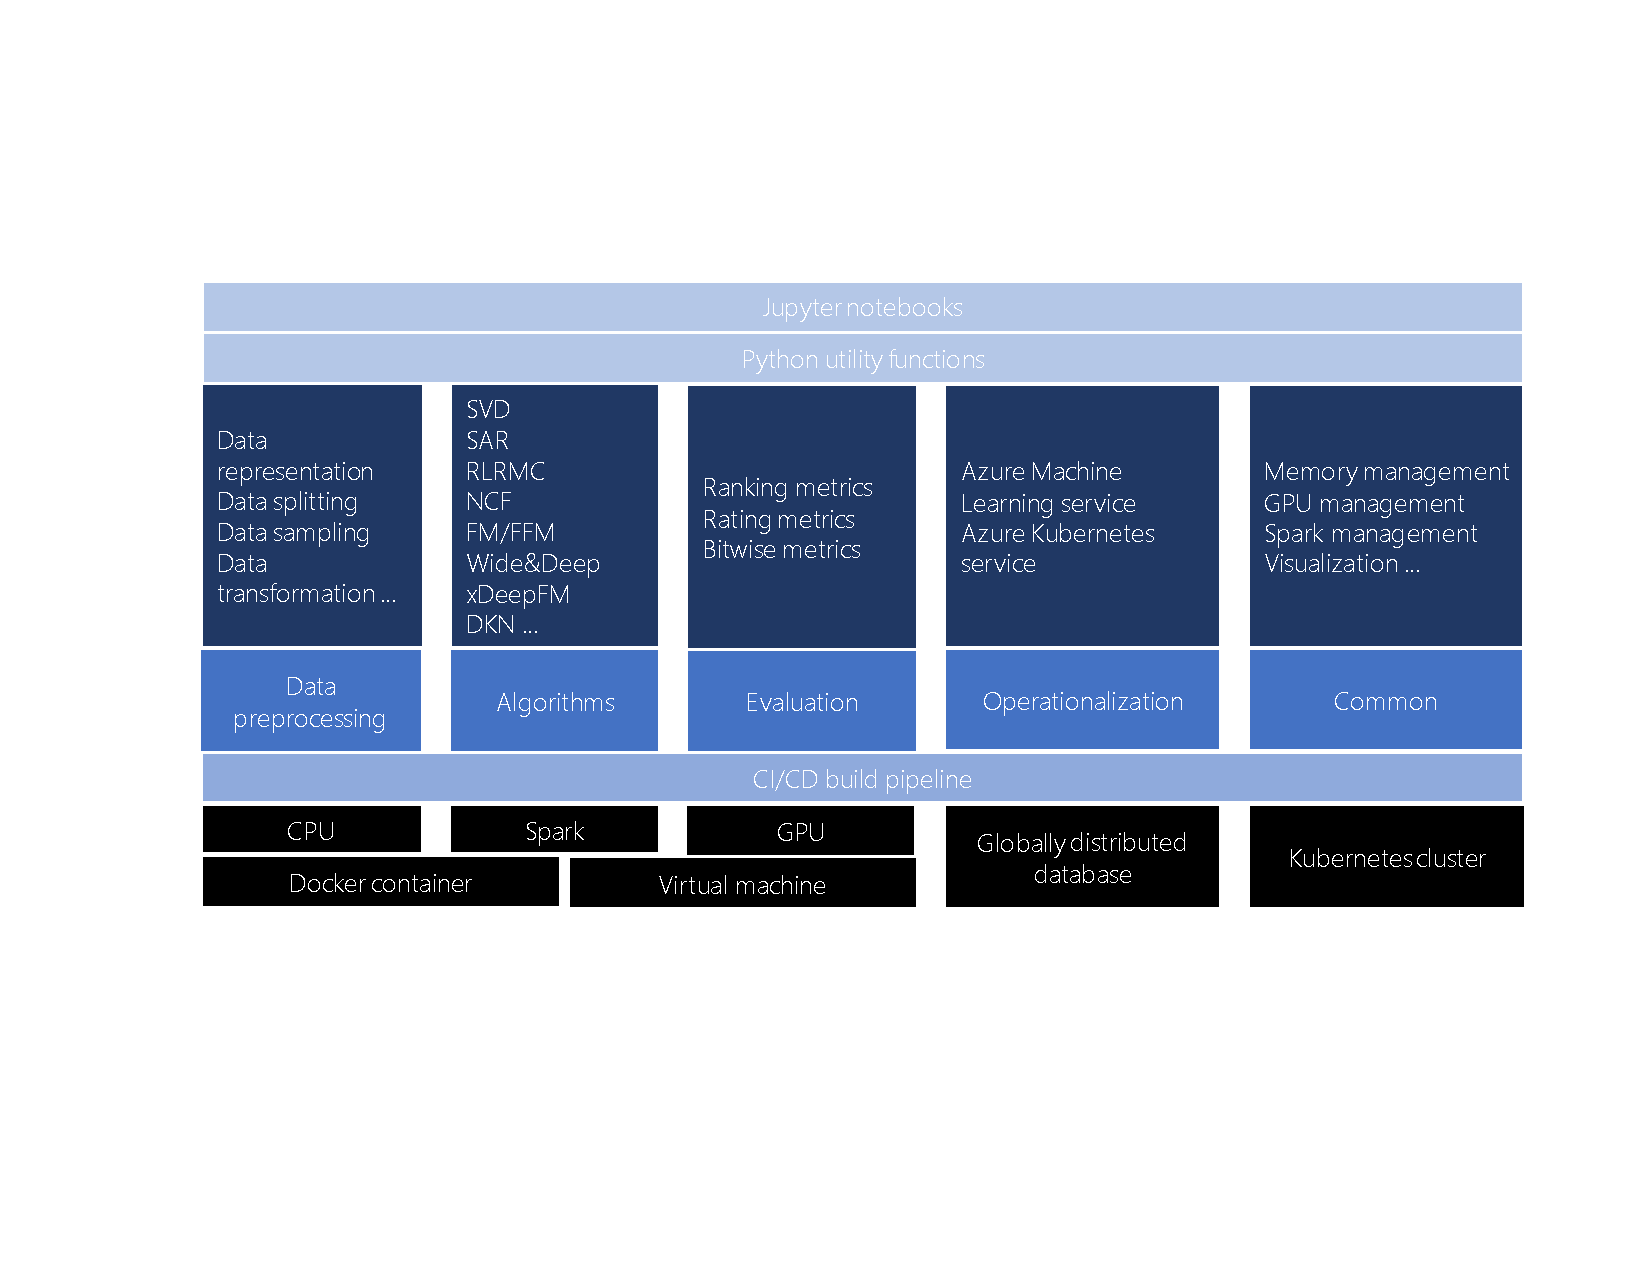
\includegraphics[width=\textwidth,keepaspectratio]{platform_diagram_crop.pdf}
  \caption{Microsoft Recommenders structure diagram. Layers from the bottom to the top support the underlying infrastructure, build pipeline, recommendation pipeline tasks, and example notebooks and utility functions.}
\end{figure}

Microsoft-Recommenders is based on best practices for building recommendation systems, which have been learned from application with production-ready systems.
As a consequence, we have followed an {\em end-to-end} approach, which is not limited to just the training of an algorithm, but encompasses the following components, typical in a recommendation pipeline:

\begin{itemize}
\item Data preparation: Preparing and loading data for each recommender algorithm
\item Model: Building models using various classical and deep learning recommender algorithms such as Alternating Least Squares (ALS) \cite{koren2009matrix} or eXtreme Deep Factorization Machines (xDeepFM) \cite{lian2018xdeepfm}.
\item Evaluate: Evaluating algorithms with offline metrics
\item Model Select and Optimize: Tuning and optimizing hyperparameters for recommender models
\item Operationalize: Operationalizing models in a production environment on Azure
\end{itemize}

Several utilities are provided in the 
reco utils folder\footnote{\url{https://github.com/microsoft/recommenders/blob/master/reco_utils}} 
to support common tasks such as loading datasets in the format expected by 
different algorithms, evaluating model outputs, and splitting training/test data. 
Implementations of several state-of-the-art algorithms are provided for self-study and 
customization in one's own applications.


\subsection{Data Preparation}

In this directory, notebooks are provided to illustrate utility functions for data operations such as data import / export, data transformation, data split, etc., which are frequent data preparation tasks witnessed in recommendation system development.

Notebook	Description
data split	Details on splitting data (randomly, chronologically, etc).
data transform	Guidance on how to transform (implicit / explicit) data for building collaborative filtering typed recommender.
** Data split Three methods of splitting the data for training and testing are demonstrated in this notebook. Each supports both Spark and pandas DataFrames.

Random Split: this is the simplest way to split the data, it randomly assigns entries to either the train set or the test set based on the allocation ratio desired.
Chronological Split: in many cases accounting for temporal variations when evaluating your model can provide more realistic measures of performance. This approach will split the train and test set based on timestamps by user or item.
Stratified Split: it may be preferable to ensure the same set of users or items are in the train and test sets, this method of splitting will ensure that is the case.
** Data transform Data transformation techniques which are commonly used in various recommendation scenarios are introduced and reviewed.

\subsection{Recommendation Algorithms}

The table below lists recommender algorithms currently available in the repository. Notebooks are linked under the Environment column when different implementations are available.

% A couple of lines only for each algorithm	mentioning the computational environment and what type (CF, hybrid etc.)

\subsubsection{ALS}


\subsubsection{SAR}

\subsubsection{LightGBM}

\subsubsection{NCF}

\subsubsection{xDeepFM}

\subsubsection{RBM}

\subsubsection{SVD}

\subsubsection{VW}

\subsubsection{DKN}

\subsubsection{FAST}

\subsubsection{RLRMC}

\subsubsection{Wide \& Deep}

In this directory, a notebook is provided to illustrate evaluating models using various performance measures which can be found in reco utils.

Notebook	Description
evaluation	Examples of different rating and ranking metrics in Python+CPU and PySpark environments.
Two approaches for evaluating model performance are demonstrated along with their respective metrics.

Rating Metrics: These are used to evaluate how accurate a recommender is at predicting ratings that users gave to items
Root Mean Square Error (RMSE) - measure of average error in predicted ratings
R Squared (R2) - essentially how much of the total variation is explained by the model
Mean Absolute Error (MAE) - similar to RMSE but uses absolute value instead of squaring and taking the root of the average
Explained Variance - how much of the variance in the data is explained by the model
Ranking Metrics: These are used to evaluate how relevant recommendations are for users
Precision - this measures the proportion of recommended items that are relevant
Recall - this measures the proportion of relevant items that are recommended
Normalized Discounted Cumulative Gain (NDCG) - evaluates how well the predicted items for a user are ranked based on relevance
Mean Average Precision (MAP) - average precision for each user normalized over all users
Arear Under Curver (AUC) - integral area under the receiver operating characteristic curve
Logistic loss (Logloss) - the negative log-likelihood of the true labels given the predictions of a classifier

 
\subsection{Model Selection}

In this directory, notebooks are provided to demonstrate how to tune and optimize hyperparameters of recommender algorithms with the utility functions (reco utils) provided in the repository.

Notebook	Description
%tuning_spark_als	Step by step tutorials on how to fine tune hyperparameters for Spark based recommender model (illustrated by Spark ALS) with Spark native construct and hyperopt package.
%azureml_hyperdrive_wide_and_deep	Quickstart tutorial on utilizing Azure Machine Learning service for hyperparameter tuning of wide-and-deep model.
%azureml_hyperdrive_surprise_svd	Quickstart tutorial on utilizing Azure Machine Learning service for hyperparameter tuning of the matrix factorization method SVD from Surprise library.
%nni_surprise_svd	Quickstart tutorial on utilizing the Neural Network Intelligence toolkit for hyperparameter tuning of the matrix factorization method SVD from Surprise library.

\subsection{Operationalization}

In this directory, a notebook is provided to demonstrate how recommendation systems developed in a heterogeneous environment (e.g., Spark, GPU, etc.) can be operationalized.

Notebook	Description
%als_movie_o16n	End-to-end examples demonstrate how to build, evaluate, and deploy a Spark ALS based movie recommender with Azure services such as Databricks, Cosmos DB, and Kubernetes Services.
%aks_locust_load_test	Load test example for a recommendation system deployed on an AKS cluster
%lightgbm_criteo_o16n	Content-based personalization deployment of a add click prediction scenario

\subsection{Utilities}

This module (reco utils) contains functions to simplify common tasks used when developing and evaluating recommender systems. A short description of the sub-modules is provided below. For more details about what functions are available and how to use them, please review the doc-strings provided with the code.

Sub-Modules
Common
This submodule contains high-level utilities for defining constants used in most algorithms as well as helper functions for managing aspects of different frameworks: gpu, spark, jupyter notebook.

Dataset
Dataset includes helper functions for interacting with Azure Cosmos databases, pulling different sizes of the MovieLens dataset and formatting them appropriately as well as utilities for splitting data for training / testing.

Data Loading
The movielens module will allow you to load a dataframe in pandas or spark formats from the MovieLens dataset, with sizes of 100k, 1M, 10M, or 20M to test algorithms and evaluate performance benchmarks.

%df = movielens.load_pandas_df(size="100k")
Splitting Techniques:
Currently three methods are available for splitting datasets. All of them support splitting by user or item and filtering out minimal samples (for instance users that have not rated enough item, or items that have not been rated by enough users).

Random: this is the basic approach where entries are randomly assigned to each group based on the ratio desired
Chronological: this uses provided timestamps to order the data and selects a cut-off time that will split the desired ratio of data to train before that time and test after that time
Stratified: this is similar to random sampling, but the splits are stratified, for example if the datasets are split by user, the splitting approach will attempt to maintain the same set of items used in both training and test splits. The converse is true if splitting by item.
Evaluation
The evaluation submodule includes functionality for performing hyperparameter sweeps as well as calculating common recommender metrics directly in python or in a Spark environment using pyspark.

Currently available metrics include:

Root Mean Squared Error
Mean Absolute Error
R2
Explained Variance
Precision at K
Recall at K
Normalized Discounted Cumulative Gain at K
Mean Average Precision at K
Area Under Curve
Logistic Loss
Recommender
The recommender submodule contains implementations of various algorithms that can be used in addition to external packages to evaluate and develop new recommender system approaches. Currently the Simple Adaptive Recommender (SAR) algorithm is implemented in python for running on a single node.


\section{Best Practices in Recommendation Systems}

Best practices of Microsoft Recommenders lie in four folds.
First, it is designed to provide {\em guidance} on 
algorithm selection under a pre-defined business or technical circumstance
Second, code design of the repository adopts best engineering practices from popular libraries like Tensorflow 
\cite{abadi2016tensorflow}, PyTorch \cite{paszke2017automatic} and LightGBM 
\cite{ke2017lightgbm}, supported with an {\em evidence-based software design} methodology 
\cite{joeglekar2018evidence}. Third, the repository
is to serve as a tool for {\em scientific reproducibility} when novel algorithm is designed and tested. And finally, the repository offers {\em space of collaboration} for the machine learning community to make
joint contributions in the recommendation realm. 






\subsection{Code Design}
\label{code-style}

We strive to maintain high quality code so as to make the utilities in the repository easy to 
understand, use, and extend. We also strive to maintain a friendly and constructive 
environment. We have found that having clear expectations on the development process 
and consistent style helps to ensure everyone can contribute and collaborate effectively.
We have published the coding 
guidelines\footnote{\url{https://github.com/Microsoft/Recommenders/wiki/Coding-Guidelines}\label{foot_code_guidelines}} 
in the wiki for the repository. Next, we describe the most important parts.

\subsubsection{Evidence-Based Software Design}
At its core, Evidence-Based Design (EBD) \cite{kembel2012architectural,joeglekar2018evidence} embodies the 
scientific method: it empowers one to ask the right questions and develop hypotheses, 
gather quantitative and qualitative data that support or disprove these hypotheses, 
and measure, share, and learn from the outcomes.

In the case of Recommenders, the evidence is gathered from extensive experience working 
with customers in real life recommendation scenarios. When there is no input from a 
customer, the second source of evidence that is used is popular machine learning
libraries like Tensorflow \cite{abadi2016tensorflow}, PyTorch \cite{paszke2017automatic},
Scikit-learn \cite{pedregosa2011scikit} or LightGBM \cite{ke2017lightgbm}.

One example illustrating EBD is the definition of the metrics interfaces in Python (not in a Spark context) and 
PySpark \cite{meng2016mllib}. The definition in Python is based on functions:

\begin{minted}{python}
    from reco_utils.evaluation.python_evaluation import rmse
    result = rmse(df_test, df_predictions)
\end{minted}

whereas the definition in PySpark is based on classes:
\begin{minted}{python}
    from reco_utils.evaluation.spark_evaluation import SparkRatingEvaluation
    rating_eval = SparkRatingEvaluation(df_test, df_prediction)
    result = rating_eval.rmse()
\end{minted}

The selection of classes in PySpark and functions in Python, instead of having a unified
interface, is derived from the EDB principle. Any machine learning practitioners
who code in Python will naturally choose a function when computing metrics, 
in a way similar to Scikit-learn \cite{pedregosa2011scikit}. By contrast, PySpark users 
will tend to code based on classes as defined in \cite{meng2016mllib}. 

\subsubsection{Test Pipeline}

The test pipeline in Recommenders is more complicated than in most machine learning
libraries \cite{abadi2016tensorflow,paszke2017automatic,pedregosa2011scikit,ke2017lightgbm}.
Apart from standard {\em unit tests} of the utilities with PyTest \cite{krekel2004pytest}, 
the Jupyter notebooks are also tested. To perform the latter tests we use Papermill 
\cite{nteract2017papermill}, which allows for programmatic execution of notebooks. The
unit tests are executed with every pull request and ensure that the utilities and 
notebooks run without error.

We have also included nightly tests consisting of {\em smoke} and {\em integration tests}
\cite{gonzalez-fierro2018beginners}. In the smoke tests, we run the notebooks with a 
small dataset or a small number of epochs to ensure that they execute without failure and that they 
output reasonable metrics. In the following example we show how 
the precision at k of SAR algorithm with Movielens 100k dataset is tested.

\begin{minted}{python}
    TOL = 0.05
    @pytest.mark.smoke
    def test_sar_single_node_smoke(notebooks):
        notebook_path = notebooks["sar_single_node"]
        pm.execute_notebook(
            notebook_path,
            OUTPUT_NOTEBOOK,
            parameters=dict(TOP_K=10, MOVIELENS_DATA_SIZE="100k"),
        )
        results = pm.read_notebook(OUTPUT_NOTEBOOK).dataframe.set_index("name")["value"]
        assert results["precision"] == pytest.approx(0.326617179, TOL)
\end{minted}

The smoke tests are a small version of the integration tests. While the integration tests
use bigger datasets with more epochs and can take from 30 minutes to several hours, the smoke tests are quicker and
will check for correctness of all the notebooks before executing the integration tests.
At the time of writing there are over 400 tests, between Windows and Linux. There are two groups of tests,
one for the {\em master branch} and one for the {\em staging branch}, which is our development branch.

The existence of a development branch, staging, is tightly related to the test pipeline. This paradigm is similar to
production and pre-production environments (master and staging, respectively).
The objective is to ensure that the code in master always works. When making a pull request, we 
do it against staging, instead of master. The nightly tests execute in staging and make sure that the new code 
works as expected and does not fail. When staging is stable, we merge it to master with a pull request.  


\subsubsection{Other Design Patterns}

We have introduced a number of design patterns which are standard in industry and well-known
in the open source community. For instance, \textit{don't repeat yourself}, \textit{single
responsibility} or the Zen of Python\footnote{\url{https://www.python.org/dev/peps/pep-0020/}}. 

The following example illustrates the pattern \textit{explicit is better than implicit}.
An implicit read function would be: 
\begin{minted}{python}
    def read(filename):
        # code for reading a csv or json
        # depending on the file extension
\end{minted}

whereas the explicit example would be:
\begin{minted}{python}
    def read_csv(filename):
        # code for reading a csv

    def read_json(filename):
        # code for reading a json
\end{minted}




\subsection{Usage and Reproducibility} %NOT SURE ABOUT THE TITLE

One of our main goals in building Microsoft Recommenders has been to enhance several aspects of research and data science processes.
In particular, we provide utilities for tasks which are common and repetitive when building recommendations pipelines.  
{\em Data preparation} is the first stage of such a pipeline and involves loading data sets in the right format and generating training, validation and test sets from it.
We provide utilities which make it simple to download the Movielens \cite{movielens}, Criteo \footref{criteo} and Wikidata \cite{wikidata} data sets. 
For example, to load 
%For example, the following code loads 
the Movielens 100K data set to a Pandas data frame
%\begin{minted}{python}
%from reco_utils.dataset import movielens
%data = movielens.load_pandas_df(size="100k", 
%    header=["UserId", "MovieId", "Rating", "Timestamp"], title_col="Title")
%\end{minted}
one uses the function \verb!movielens.load_pandas_df()! from the \verb!reco_utils.dataset.movielens! module.
To load the data to a PySpark data frame the syntax is similar and uses the function \verb!movielens.load_spark_df()!.

Splitting a data set can also be done in one line 
with the \verb!reco_utils.dataset.python_splitters! module.
%For example, the following code performs two types of 
For example, the function 
\verb!python_random_split()! splits by random sampling 
and the function \verb!python_chrono_split()! by splitting each user"s data according to the timestamp. 
%\begin{minted}{python}
%from reco_utils.dataset.python_splitters import python_chrono_split, 
%    python_random_split
%data_train, data_validate, data_test = python_random_split(data, 
%    ratio=[0.6, 0.2, 0.2])
%data_train, data_test = python_chrono_split(data, ratio=0.7, 
%    filter_by="user", col_user="UserId", col_item="MovieId", 
%    col_timestamp="Timestamp")
%\end{minted}
There are also methods for stratified splitting (by user or item) and chronological splitting without stratification. 
There are versions of the splitter methods for both Pandas and PySpark.

Training any of the algorithms included in the repository is also straightforward. To this end, we use an interface similar to Scikit-Learn \cite{pedregosa2011scikit}, 
with algorithms defined as classes implementing \verb fit() and \verb predict() methods. For example, training a Neural Collaborative Filtering \cite{he2017neural} model
can be done as follows:
\begin{minted}{python}
    model = NCF(n_users=n_users, n_items=n_items, n_factors=4, n_epochs=100,
        layer_sizes=[16,8,4], batch_size=256, learning_rate=1e-3)
    model.fit(data_train)
    preds = [[row.userID, row.itemID, model.predict(row.userID, row.itemID)]
        for (_, row) in data_test.iterrows()]
\end{minted}

Another modular part of the recommendation process is the evaluation of metrics between two data frames consisting of users, items and numerical values 
(predicted vs. ground truth). There is a distinction between rating metrics (such as mean squared error and accuracy) and ranking metrics 
(such as top-k precision and recall). For example, computing root mean squared error is done using 
the \verb!rmse()! function from the \verb!reco_utils.evaluation.python_evaluation! module, 
or the \verb!rmse()! function in the \verb!SparkRatingEvaluation! class from \verb!reco_utils.evaluation.spark_evaluation!.
%\begin{minted}{python}
%from reco_utils.evaluation.python_evaluation import rmse
%eval_rmse = rmse(data_test, predictions, col_user="UserId", 
%    col_item="MovieId", col_rating="Rating", col_prediction="Prediction")
%\end{minted}
 
These interfaces hide all the implementation details of the algorithms involved, while providing access to the necessary parameterization.
In this way, a recommendation process can be completely replicable and reproducible from beginning to end. Furthermore, any randomization 
which is part of data processing and evaluation is exposed to the user with seed parameters, thus enabling fair comparisons between the results of different algorithms
on the same data. 


\subsection{Collaborative development paradigm} %NOT SURE ABOUT THE TITLE
Majority of the code assets in Microsoft Recommenders are hosted on Github. The whole life cycle of its development is transparent to the open source community. Codes and notebooks examples were contributed by developers, researchers, and data scientists from industrial organizations and academic research institutes. Such collaborative paradigm is supported mainly by 1) \textit{the unified CI/CD build pipeline that runs unit/smoke/integration tests and nightly builds to guarantee the adoption of high-quality codes}, 2) \textit{the coding principles that standardize the conventions applied in the notebook examples as well as the utility functions}. For instance, in contributing a new asset (either an example notebook or a utility function) to the repository, one takes the following steps
\begin{enumerate}
    \item Clone the repository to a local system and set up the development environment
    \item Develop notebooks and/or utility functions in a new branch that is based on the ``staging'' branch, push the new codes to the remote repository, and create a pull request for merging the codes to the "staging" branch
    \item The code committers are requested to follow the test-driven design principle so that unit tests for the notebooks/utilities should be developed together with the submitted codes. The freshly committed codes in the pull request are executed through a set of testings in the CI/CD pipeline hosted by using the cloud service, to guarantee that they run without failures.
    \item All participants of the repository are allowed to take part in the code review that may not be effectively captured by testing, (e.g., coding style checking as aforementioned in the section of \nameref{code-style}).  
    \item The codes are merged if all the testings pass and review comments are resolved
\end{enumerate}

The ease of collaboration in Microsoft Recommenders is extendable to the enteprise-grade development. With the help of the best practice examples that cover the entire spectrum in the end-to-end pipeline of a recommender architecture, data scientists, developers, and researchers can harmoniously work out a minimum viable product, which can be easily transformed into productionized pipeline by scaling up or out the underlying computing/data storing infrastruture and build pipeline. For instance, the combination of versioning tool like Github and CI/CD pipeline on a single node machine can be extended to industry-level production system like Databricks \footnote{\url{https://databricks.com/}} and Azure DevOps \footnote{\url{https://azure.microsoft.com/en-in/services/devops/}} for production use.

\section{Lessons Learned from Building Real-World Systems} 

The core development team of Microsoft Recommenders have collaborated with data scientists and engineers 
in various industrial verticals, on production-ready recommendation systems used for different scenarios. 

%\subsection{Challenges in Bringing Recommendation Systems to Production}
%In general, challenges in building a real-world system lie in the following aspects that include but are not limited to algorithm development. 
Some of the common challenges %faced by developers of recommendation systems in practical design and implementation 
are the following. Model training and retraining every day is usually crucial to real-world applications like e-commerce where the volume and dynamics of training data change dramatically. Hyperparameters of a recommender model, especially that used for content-based recommendation scenarios, needs to be fine tuned properly in order to make sure the model delivers good performance.
Real-time model or recommendation results serving should meet the engineering specifications determined from business requirements. An end-to-end recommendation pipeline may consist of various computing framework (e.g., distributed computing cluster, GPU, etc.) where computing resources should be used effectively and economically. 
The health status of a recommender system should be well managed, and online monitoring mechanism is therefore needed such that break points of the entire pipeline is observable. 
Offline evaluation is often used for selection of algorithm, in comparison to baseline models, while it is always recommended to perform online evaluation by using A/B testing and/or multi-armed bandit for fairly evaluating a recommender system. 
Finally, a recommender system can be restricted by business rules (e.g., country-specific legislation, seen items are allowed to be recommended only a certain amount of times, if it is summer a jumper should not be recommended, etc) to make the recommendation results comply.

%\begin{itemize}
%    \item Model training and retraining in time is usually crucial to real-world applications like e-commerce where the volume and dynamics of training data change dramatically. This requires iterative optimization for model implementation as well as architecture construction.
%    \item Hyperparameters of a recommender model, especially that used for content-based recommendation scenarios, needs to be fine tuned properly in order to make sure the model delivers good performance. 
%    \item Real-time model or recommendation results serving should meet the engineering specifications determined from business requirements. 
%    \item An end-to-end recommendation pipeline may consist of various computing framework (e.g., distributed computing cluster, GPU, etc.) where computing resources should be used effectively and economically. 
%    \item Health status of a recommender system should be well managed, and online monitoring mechanism is therefore needed such that break points of the entire pipeline is observable.
%    \item Offline evaluation is often used for selection of algorithm, in comparison to baseline models, while it is always recommended to perform online evaluation by using A/B testing and/or multi-armed bandit for fairly evaluating a recommender system.
%    \item A recommender system is restricted by business rules like country-specific legislation (e.g., seen items are allowed to be recommended by only a certain amount of times, if it is in summer a jumper should not be recommended, etc) to make the recommendation results comply.
%\end{itemize}

%\subsection{Reference Architectures}
%
%To effectively mitigate most (if not all) of the aforementioned challenges, 
In response to some of these issues, 
Microsoft Recommenders provides two reference architecture designs for building production-grade systems. 
%\subsubsection{Batch-Mode Recommendations}
A \textit{batch-mode recommendation architecture} refers to a pipeline where a recommender model is built with the input data flow, and the recommendation results from that model are generated successively. In industrial recommender system where a collaborative filtering typed algorithm is used, this kind of architecture is highly effective. This is because the batch-mode pipeline hides the latency in using a model to score items and produce the top-k recommendations, by pre-caching the recommendation results into a database. In the operationalization example available in the Recommenders repository, 11,000 request units per second is achieved in a recommender system with minimal sized machines on cloud service. 
%To build a model with desirable performance by using an optimal budget, hyper parameter tuning techniques like Bayesian Optimization \cite{snoek2012practical} and Neural Architecture Search \cite{zoph2016neural} are often used. In the example notebooks shown in the Recommenders repository, applying an intelligent hyper parameter tuning technique can reduce time spent on parameter searching dramatically \footref{model_select}. 
For meeting the compliance requirement, usually post-filtering logics are incorporated in the pipeline to refine the recommendations.

%\subsubsection{Real-Time Model Serving}
\textit{Real-time model serving} refers to an architecture where attributes of users and items, contextual information, etc., are used in model building. In this scenario, a real-time model serving scheme is usually considered given the difficulty of pre-computing all possible recommendations for different feature and context combinations. Compared to the batch-mode recommendation, model management in this scenario is specially importance because a pre-trained model is re-used for scoring and item ranking. Depending on business requirements, engineering specifications, and model complexity, computing resources for model serving should be scalable and configurable for both computational efficiency and cost saving purpose. Nowadays, Kubernetes cluster is used as the industrial main stream for model serving \cite{bernstein2014containers}. Another reference architecture that illustrates the use of LightGBM model \cite{ke2017lightgbm} for real-time model serving, built on top of the Spark framework, is demonstrated in the Azure documentation. \footnote{\url{https://docs.microsoft.com/en-us/azure/architecture/example-scenario/ai/scalable-personalization}}


\section{Conclusion}

Our main objective in building Microsoft Recommenders has been to make the processes of 
doing research or data science on recommendation systems more productive.
We have had experience with several projects involving recommendation systems 
in enterprise settings. We have observed significant productivity gains by using the repository,
which amounted to speeding up the implementation time of a new algorithm or a new recommendation 
system by 10 times or more than before.


\section*{Acknowledgments}
\bibliography{references}
\bibliographystyle{plain}

\end{document}
